\chapter{Introduction}
\label{chapter:introduction}


\chapterprecishere{``Begin at the beginning,'' the King said gravely, ``and go on till you come to the end: then stop.''\par\raggedleft--- \textup{Lewis Carroll}, Alice in Wonderland}
\chapterhung

This book examines context while applications access their configuration settings.
\intro[context]{Context} includes all factors that influence an application's configuration settings, for example, information about geographical locations, installed packages, hardware configurations, network connections, and configuration settings of the system.
If software better adapts its behavior according to its context, we call it more \intro[context awareness]{context aware}~\cite{alegre2016engineering}.
Applications tend to be adaptable by \empha[configuration setting]{configuration settings}.
\intro[context-aware configuration]{Context-aware configurations} are configuration settings in accordance with their context.

Many behavioral aspects are not fixed at compile-time but are determined later by reading configuration settings.
Applications access configuration settings from configuration files, environment variables, command-line options, etc.\ at run-time.
We subsume these \empha[configuration sources]{configuration sources} under the term \empha{execution environments}.
Fetching configuration settings from the execution environments is called \empha{configuration access}.

Previously, concerns about context mainly have been addressed with workarounds and ad hoc solutions from both developers and system administrators.
Here we address these concerns in a comprehensive and structured way.
The book describes a holistic and unified context-aware configuration access.
We aim at better abstractions at the system-level to improve user experience.

We write explanations and definitions of terms in \emph{italics}.
We bootstrap from minimal explanations in this chapter to definitions later.
For example, dissociation of configuration settings to input and sensor data is given in \defref{configuration-setting}. %page number wrong!
The index on page~\pageref{index} contains page numbers for all these terms.

In the rest of this chapter, we discuss the challenges, the goal, the solution, the structure, research questions, and the contributions of the book.








\section{Challenges in Configuration Access}
\label{sec:introduction-motivation}

Configuration access appears to be straightforward:
Applications need to read the execution environments and prepare these configuration settings to be accessed in the source code.
System administrators, however, experience many surprises around configuration access on a daily basis.
Na\"{i}ve ways to access configuration, which are typically used, are not safe and do not take context into account.


In the systems community, problematic configuration settings are well-known as \empha[misconfiguration]{misconfigurations}~\cite{yin2011empirical,su2007autobash,attariyan2010automating,xu2015systems}.
Misconfigurations are a major cause of system failures~\cite{wool2004quantitative,oppenheimer2003internet,pertet2005causes}.
As studies show~\cite{rabkin2011static,oppenheimer2003internet,yin2011empirical,mahajan2002bgp}, system administrators need to spend much time to fix misconfigurations.
In this section we describe challenges we tackle in this book.


\subsection{Stakeholder's View}

Three different \intro[stakeholder]{stakeholders} participate in configuration accesses.
Each stakeholder has different interactions and problems with configuration settings and their context~\cite{raab2017introducing}:

\begin{description}
\item[Developers] implement configuration access in their applications and do not foresee every possible context influencing the application.
They need to provide interfaces for configuration settings to be used by other stakeholders.
For them, context is mainly the system the application is running on.

\item[System administrators] prefer direct, precise, and concise ways to change configuration settings.
Therefore, their typical interface to configuration settings are low level, such as configuration files~\cite{barrett2003system,barrett2004field,haber2007design,velasquez2008designing,zhang2014configuration}.
For them, context is mainly the system's settings and other applications' settings.
Because constraints on configuration settings concerning context tend to be too complex for manual consideration, system administrators easily miss considering some context.
They wish to get concise error messages if configuration settings are invalid, for example, conflicting with context.

\item[End users] expect applications to be automatically adapted to their context.
Furthermore, they want to customize applications to their special needs, which can be different in different contexts.
For end users, context is everything relevant for their interactions with applications.
\end{description}

Although the stakeholder's views are different, the same consequences for configuration access apply:
Context puts constraints on the configuration settings, and it is problematic if these constraints are violated.

\subsection{System's View}

\citet{yin2011empirical} discovered that \enquote{a majority of misconfigurations (\p{70.0}$\sim$\p{85.5}) are due to mistakes in setting configuration}.
The other \p{14.5}$\sim$\p{30} of \enquote{misconfigurations are caused by software compatibility and component configuration}.
A main contributor to misconfigurations are configuration settings clearly violating syntactic or semantic rules (\p{38.1}$\sim$\p{53.7}).
Such errors can be avoided with configuration validation.
\intro[configuration validation]{Configuration validation}, or \intro[validation|see{configuration validation}]{validation} in short, rejects invalid configuration settings by checking syntactic and semantic rules.
Validation is present in end-user interfaces, but hardly in the interfaces system administrators use.
For system administrators, validation only occurs while restarting the application---putting the system at a high risk.

The system administrator's interfaces are confusing, too~\cite{barrett2003system,barrett2004field}.
System administrators easily confuse syntax because applications have many subtle differences in configuration file formats~\cite{barrett2004field}.
Even more traps for system administrators are hidden behind the interfaces.
\citet{xu2013blame}~showed that system administrators are not to blame.
Instead configuration access code in the applications is leading to unexpected behavior and crashes.
Only in \p{7.2} to \p{15.5} of cases error messages pinpoint the error~\cite{yin2011empirical,raab2017challenges}.

\begin{example}
\label{ex:introduction-openldap-crash}
OpenLDAP has the configuration setting ^listener-threads^.
Its documentation says: \enquote{The default is 1 and this is typically adequate for up to 16 CPU cores. The value should be set to a power of 2.}
OpenLDAP's documentation does not mention:
\begin{itemize}
\item how to correctly use this setting for more than 16 CPU cores,
\item that ^slapd^ will reduce the value of ^listener-threads^ to the next number that is \enquote{a power of 2}, nor
\item that ^slapd^ will crash with values above 16~\cite{xu2013blame}.
\end{itemize}
Such behavior is a trap for system administrators.
\end{example}



Now that we have established that applications are vulnerable against misconfiguration, we elaborate on the challenges in providing configuration validation.
Problems of the application are located in the configuration access, i.\,e., along the data flow of configuration settings from the configuration parser to their use in the application.
\citet{xu2013blame}~investigated the configuration access in seven applications.
The results show that configuration settings are not considered as input to the application and not validated systematically.
Even worse, sometimes there are checks and transformations that lead to surprises in behavior.
We will subsume all descriptions of the configuration access as \intro{configuration specification}.
Their study shows that the available implementations of configuration specifications are woven into the application's source code.
As a result, configuration specification cannot easily be separated from the source code nor moved to a separate tool.
Applications validate their settings only at startup, or even later~\cite{xu2016early}.
Checking at startup is already too late:
Failures at startup can cause outages.

\subsection{Context and Beyond}

Currently applications, which have configuration validation, typically only check consistency within their own settings.
They hardly include checks with respect to their context.
In particular, system-wide settings or others applications' settings are often prone to mismatch.
\intro[context specification]{Context specifications} describe context relevant for configuration settings.
As we will see later, context specifications are an important part of configuration specification.
For example, context information about network settings and installed packages are easily available within the network and package managers.
Such context information, however, is not readily available within applications.
This implies that configuration validation within applications fails to include such context.


A survey from \citet{xu2015systems} gives insights about system approaches to tackle misconfiguration.
It shows (by absence of the topic) that most research does not include context of configuration settings, despite empirical research that shows its importance:
\enquote{a large portion (\p{46.3} to \p{61.9}) of the parameter misconfigurations have perfectly legal parameters} (i.\,e., configuration settings)~\cite{yin2011empirical}.
If the configuration settings are valid from the view of the application but still invalid in the system, it means that some requirement or context influencing the application was not considered.

\begin{example}
\label{ex:workplaces-proxy}
People and their devices often change between different workplaces.
Their computers need various network settings where each of them requires different proxy and printer settings.
If the user changes workplace, the proxy and printer settings need to be changed according to the network settings.
Without changing the proxy, the browser will not be able to connect to the Internet.
Configuration settings that are perfectly valid in one situation are invalid in another situation.
\end{example}

Not all misconfigurations with valid settings are due to context unawareness:
The second half are violated requirements such as performance, privacy, or security.
These factors decide about \empha{suitability} of configuration.
\begin{example}
MySQL has the configuration setting ^AutoCommit^:
\enquote{But when the user set[s] this parameter to be \texttt{True}, she was not aware of the performance impact}~\cite{yin2011empirical}.
In this example, the performance is a disregarded requirement.
\end{example}

Applications can avoid misconfigurations if their configuration specification would take context and requirements into account.
In some cases, we can avoid any manual interaction and calculate \empha[default value]{default values} from context information.
We see such software rarely because of the applications' inability to inquire context.
System administrators would benefit if the configuration specifications use such context information or at least tell if they are inconsistent.%
{\parfillskip=0pt plus .8\textwidth \emergencystretch=.5\textwidth \par}

Usability improvements due to context is not limited to system administrators but applies to all users.
\citet{khalil2005context} conducted a study where all users found context-aware configuration (very) useful.
They learned that in \p{89} of cases the mapping between activities and settings was consistent for individual users.
In the study, context-aware configuration improved satisfaction, even if deduced settings sometimes were not appropriate.
For example, a participant stated:

\begin{quote}
``I like how it changes state without you having to tell it to. I always forget to turn my cell [off] in class and turn it on after.''
\end{quote}

Despite these long-known advantages of context-aware configuration, developers hardly implemented them in their applications.
Before this work, it was not even known why developers failed to implement these techniques.

\subsection{Configuration Integration Problem}

\label{sec:introduction-configuration-integration}
Developers find it challenging to consider configuration settings and specifications if they belong to other applications.
Inter-woven implementations of configuration specifications, missing context information within applications, and different configuration file formats are symptoms of the same problem.
Figure~\ref{fig:cursituation} shows:
If $n$ applications read configuration settings and specifications of every other application and the system, we need at least $n*(n+1)$ ways to extract configuration settings and specifications.
The same applies to tools for system administrators.
It is unfeasible to take the hurdle to implement access to all configuration settings and specifications.
We call the problem \linebreak \intro{configuration integration problem}\footnote{Based on the name given by \citet{keidel2016ide} \enquote{IDE portability problem}.}.

\begin{figure}[htp]
\centering
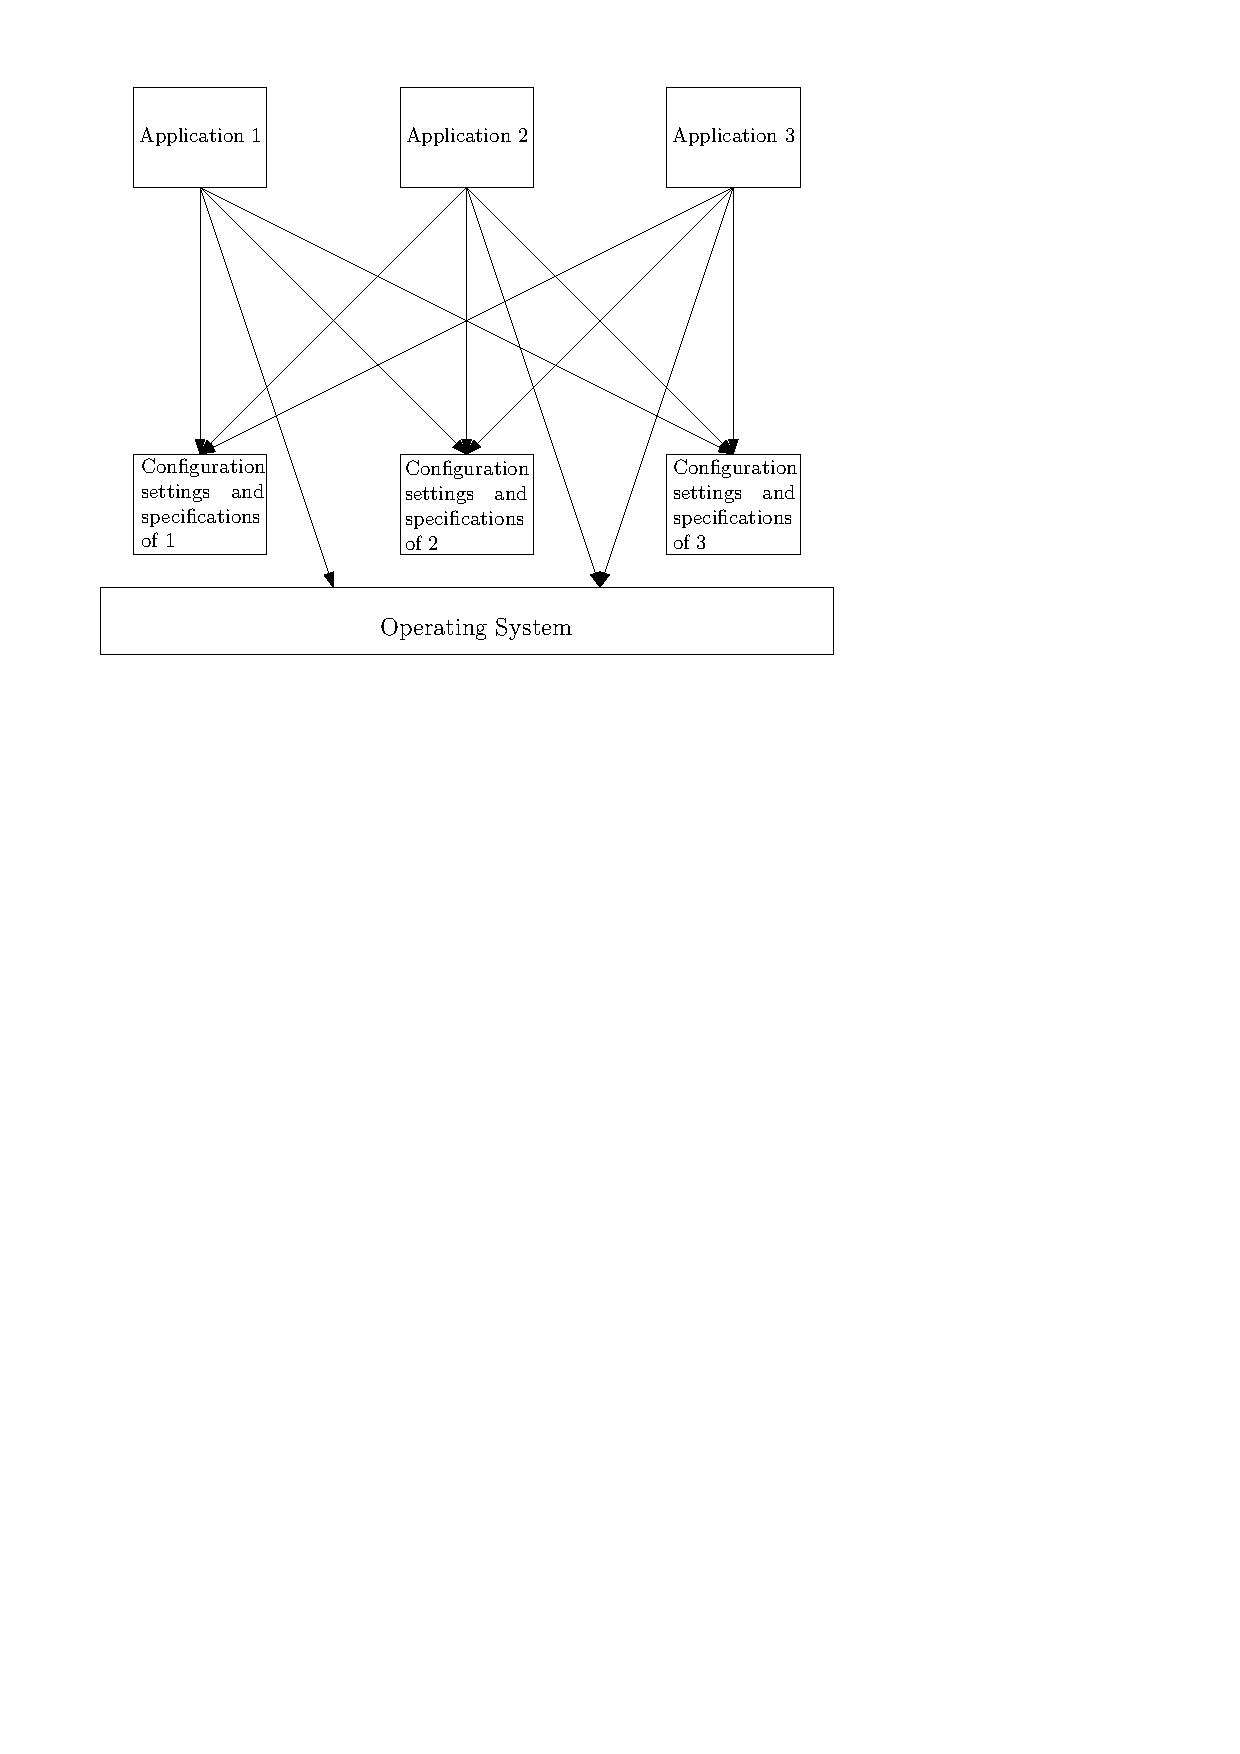
\includegraphics[width=\columnwidth]{cursituation}
\caption[Current Situation.]{Current situation: For $3$ applications and $4$ sources of configuration settings and specifications, we need $3*4=12$ configuration accesses.}
\label{fig:cursituation}
\end{figure}

Because of the configuration integration problem, applications do not use configuration settings and specifications from other parts of the system.
Even applications, for that other configuration settings are highly relevant, often have no awareness of this context.
The configuration integration problem hinders us to create better tools badly needed by system administrators.
Furthermore, the configuration integration problem restrains the context awareness of applications, reducing usability.
\begin{example}
OpenLDAP is unable to determine the value for ^listener-threads^ because it lacks context information about the number of CPUs present in the system.
\end{example}





\section{Methodology, History, and Goals}

The aim of the book is to find a system-oriented, computer-language-based solution to the configuration integration problem.
In this section we discuss the methodology, history, gaps, goals, and limitations.

\subsection{Methodology}

Before we start designing a formal language, we must understand precisely what we want to express in this formal language.
We did an in-depth gap analysis and conducted empirical studies to better understand the configuration integration problem.
From these unveiled requirements we started to design a framework and a formal language.

We used the methodological framework \enquote{theory building from cases}~\cite{easterbrook2008selecting,eisenhardt2007theory} with different methods embedded:

\begin{enumerate}
\item an observation report, to learn about fundamental requirements,
\item a questionnaire survey, to learn about goals of potential users, and
\item a source code analysis, to validate statements of potential users.
\end{enumerate}

To countervail weaknesses of individual methods, we mixed them in a way to minimize the threats of validity of our overall results~\cite{ihantola2011threats}.
There is a huge gap between empirical studies of problems and software requirements.
We tried to fill it with experience, but it would be unrealistic to claim that there is no room for improvements in the requirements.
With the unveiled requirements, we redesigned and reimplemented a framework, called \elektra{}, and evaluated it.


\subsection{\textsc{Elektra}}

In this book we present the framework \elektra{} that consists of several parts:

\begin{enumerate}
 \item The library \elektra{Lib} is a \empha{configuration library}, which means it provides access to configuration settings.
 It already existed before the book was started.
 \item The modular \empha{configuration specification language} \elektra{Spec} is the main contribution of this book.
 \item Several tools and frontends are built on top of \elektra{Lib}.
       In this book we will mostly discuss the code generator \elektra{Gen}.
\end{enumerate}

\begin{wrapfigure}{r}{0.5\textwidth}
\centering

\includegraphics[width=2cm]{logo}
\caption{Elektra's Logo.}
\label{fig:logo}
\end{wrapfigure}

\elektra{Lib} is a library that aims to provide unified access to configuration settings and specifications as found in the execution environment.
It works similar to a virtual file system but is based on key-value pairs.
\elektra{Lib} enables introspection for both configuration settings and specifications.
Developers use the configuration specifications to externally specify their configuration access, validations, and default value calculations.
\empha[plugin]{Plugins}, implementing configuration access, enforce these configuration specifications.
The idea of the plugins is to provide system-level dependence injection~\cite{raab2017challenges}.



\subsection{\textsc{Elektra}'s History}

The development of \elektra{Lib} started in 2004, sponsored by IBM at that time.
The author of this book joined in the same year.
A community, called \emph{\elektra{} initiative}, gathered around the source code repository of \elektra{Lib}.
Initially the initiative only aimed at the straightforward idea to unify \empha[application programming interface (API)]{application programming interfaces (APIs)} for \empha[configuration access API]{configuration access}.
From its beginning, \elektra{} was \empha[free/libre and open source software]{free/libre\footnote{The word ``free'' here is interpreted with the meaning of the word ``libre''. The term FLOSS is designed for the purpose of not taking political position between free software and open source software, see also \url{https://www.gnu.org/philosophy/floss-and-foss.en.html}.} and open source software (FLOSS)}.
\elektra{Lib} started by introducing an API with many language bindings.
The bindings were contributed by different people who felt an API, to unify configuration settings, is important.

The idea of introducing a configuration access API was not new:
Most proprietary software systems already had similar APIs for a long time.
Nevertheless, it was clear that there was no portable configuration library available to be used for typical FLOSS applications.
For example, the configuration libraries X/Q/GSettings, KConfig, dconf, plist, and Windows Registry are tied to their respective platforms.

Grave mistakes in initial versions led to several redesigns of the API.
Due to that, \elektra{} lost many FLOSS users.
Despite different efforts to change the situation, rather companies than FLOSS software developers used \elektra{}.
Focus was often at patching applications that led to quality problems in \elektra{Lib} itself.
Unfortunately, redesigns had new flaws and unnecessary features were introduced.
In particular, developers started implementing a daemon, which did not offer advantages but introduced many complications.
Reimplementing security features of the operating system frustrated developers, who then left.
The \elektra{} initiative was in a deep crisis that escalated in 2006 when IBM canceled their sponsoring.
On the positive side \elektra{} was well-known and had supporters~\cite{raab2017challenges}.%
{\parfillskip=0pt plus .8\textwidth \emergencystretch=.5\textwidth \par}

In 2007 the author of the book continued the work on \elektra{} mostly alone and thus progress was at a slow pace.
In 2012 the author did a major cleanup and in 2014 the author restarted the initiative.
More than ten students supervised by the author started to work on topics related to \elektra{} for their Bachelor's and Master's theses.
The author of the present book started to lead this revived \elektra{} initiative.
The newly formed initiative is referred as ``we'' in the following paragraphs about history.
Additional contributors, early adopters, and package maintainers also joined the effort.
A separation of what was done by the author follows much later in \secref{elektra-metrics} after we had explained all parts of \elektra{} in detail.

The new lead shifted the goals towards a more technical solution to mitigate the configuration integration problem:
We focused on inventing new abstractions other configuration access APIs did not have.
We oriented towards the highly competitive market of configuration libraries.
As unique selling point our abstractions forced less ideology onto users because \elektra{} avoids prescribed configuration validation techniques or configuration file formats.
In a first step, this was achieved by introducing different backends, chosen by users at run-time.
An implementation providing only a single backend for the whole system proved to be too limited:
Individual applications cannot customize their backends for their own needs.
We implemented a layer similar to a virtual file system, which enables applications and system administrators to mount configuration files~\cite{raab2008thesis}.
Furthermore, dependences in the core made \elektra{} unattractive.
To solve this problem, we modularized \elektra{}~\cite{raab2010thesis} so that users can select exactly the features they need~\cite{raab2017challenges}.%
{\parfillskip=0pt plus .8\textwidth \emergencystretch=.5\textwidth \par}

Such changes made part of the software more complicated.
At first, we provided too little documentation for newcomers to grasp the abstraction mechanisms~\cite{raab2010thesis}.
Then we started to put efforts into rebuilding the community by overhauling documentation, introducing more regression tests, writing tutorials, and designing a new website.
We succeeded by other FLOSS initiatives willing to use \elektra{}, and \elektra{} being packaged for many distributions~\cite{raab2017challenges}.%
{\parfillskip=0pt plus .8\textwidth \emergencystretch=.5\textwidth \par}


\subsection{Scientific Gaps}

Now back from the history of \elektra{} to this book.
When the book started in 2013 (shortly before reviving \elektra{}) the author searched for scientific gaps to be solved to explain the previously mentioned phenomena.
The following scientific gaps refer to the situation at that time.

The research topic of \empha[context-aware application]{context-aware applications} is well-known~\cite{riva2006unearthing,baldauf2007survey}.
\empha[context-oriented programming]{Context-oriented programming} is a novel programming paradigm that aims at programming-language support to implement context-aware applications~\cite{keays2003context,kamina2014context,appeltauer2009contextcomparision,hirschfeld2008context}.
It allows us to describe context, in which the application is situated in, as state of the application.
Context-oriented programming languages did not consider the execution environment and did not have desired performance characteristics.

Configuration accesses did not have support for context awareness.
Na\"{i}ve ways to implement context awareness led to the problems mentioned earlier.
Accounting context in configuration access differs in some aspects from earlier work on context-\linebreak{}oriented programming:
{\parfillskip=0pt plus .8\textwidth \emergencystretch=.2\textwidth \par}


\begin{enumerate}
\item We cannot start sensing context within the application before it starts up.
Nevertheless, the configuration access at startup must be efficient.
\item We shall not assume developers to know every possible context during development.
\item We shall not assume developers to rewrite large-scale software for context-aware configuration.
\item Improved simplicity for configuration access is essential:
For developers the status-quo is a viable option.
\end{enumerate}


Because of these reasons, earlier work of context-oriented programming could not be applied.
There was no concept telling us how context-oriented programming can be used without large overhead~\cite{raab2014program}.
Neither did the previous approaches permit multi-threading~\cite{raab2015global} nor multi-process~\cite{raab2016persistent} configuration access.
No previous surveys about context awareness for configuration access were done.
Therefore, despite developing \elektra{} since nearly 10 years, we were unaware about some expectations, goals,\linebreak and challenges.%
{\parfillskip=0pt plus .7\textwidth \emergencystretch=.2\textwidth \par}

\empha[configuration specification language]{Configuration specification languages}~\cite{gunther2012software,berger2013survey,hewson2011modelling,magableh2010primitive,friedrich1999consistency} did not have configuration access in their scope.
The configuration specification languages did not have capabilities for local configuration validation of configuration files~\cite{raab2015safe}.
Furthermore, they were usually not as extensible as needed for the needs of the many different applications.
For example, they did not have a practical way to be extended with application-specific run-time checks.
We found a scientific gap for a configuration specification language that is easy to use for simple tasks but can be extended to domain-specific, complex tasks.%
{\parfillskip=0pt \par}

Configuration libraries did not have an abstraction for programmable configuration access~\cite{raab2017challenges,raab2016improving}.
Research was needed to investigate the solution space.
Another scientific gap was the missing way to specify requirements used at configuration access~\cite{raab2016improving}.
Previous solutions had specifications that generated configuration files causing problems in a bidirectional work flow.

\citet{behrang2015users} found ill-tested applications in which errors caused by co-evolution will not be automatically detected by a test suite.
Instead configuration settings, that were in fact not used by the application anymore, were still presented to users.
\citet{jin2014configurations} found configuration settings present in the source code but not shown to the users, for example ^autoadmin.append_emailaddr^ in Firefox.
We had to find a configuration specification language that eliminated such inconsistencies.

\citet{holland2001nofutz}~defined \empha{futzing} to denote \enquote{tinkering or fiddling experimentally with something.}
Instead of having a straightforward way to achieve a goal, the user needs to use trial-and-error methods.
With \intro[no-futz computing]{no-futz computing} \citet{holland2001nofutz} mean \enquote{that futzing should be allowed, but should never be required.}
Many situations, however, required system administrators to futz, for example, to reverse engineer configuration access code to know the state of configuration settings~\cite{holland2001nofutz}.

Last but not least, no method existed that allowed applications without any modifications in the source code to have context-aware configuration access~\cite{raab2016unanticipated}.
Or more generally, there was no way to apply context-oriented programming in another way than rewriting applications.


\subsection{Goals}


Let us elaborate on our aim to solve a computer-language design problem with the goal to improve on the configuration integration problem.
\elektra{} is a vehicle to study candidate techniques whether they enable developers to build a futz-free configuration system.
To validate if \elektra{} mitigates the configuration integration problem, we define the following goals.
As precondition, we must understand the requirements by looking at the developer's challenges:

\begin{restatable}[Requirement]{goal}{goalRequirements}
\namedlabel{goal:requirements}{Requirement}
A goal of this book is to unveil requirements by empirically analyzing how applications access configuration settings and why developers programmed it that way.
\end{restatable}

With these requirements, the next goal can be tackled:

\begin{restatable}[Abstraction]{goal}{goalAbstraction}
\namedlabel{goal:abstraction}{Abstraction}
We create an abstraction by designing the configuration specification language \elektra{Spec}.
This abstraction shall enable users to reduce effects of the configuration integration problem by unifying configuration access, simplifying configuration validation, and enabling context awareness.
\end{restatable}

Then we want to implement the abstractions defined in \elektra{Spec} within the \elektra{} framework.
With this better abstraction, we grapple the next goal:

\begin{restatable}[Context]{goal}{goalContext}
\namedlabel{goal:context}{Context}
We aim at a run-time system that automatically chooses the best suitable configuration settings with regard to the context.
We want to enable users to consistently manipulate and introspect which configuration settings an application receives.
Making changes in configuration settings shall be futz-free.
\end{restatable}

If new contexts and requirements arise, we ideally only need to change configuration settings and specifications---without any need to modify the source code of applications.
The best run-time system is of little benefit if it is used incorrectly, thus we need to fulfill:

\begin{restatable}[Frontend]{goal}{goalFrontends}
\namedlabel{goal:frontends}{Frontend}
We aim at a context-aware, type-safe frontend that mitigates problems unveiled before.
The effort to let applications participate with this run-time system shall be kept at a minimum.
\end{restatable}

\subsection{Limitations and Assumptions}

In \empha[configuration management]{configuration management}~\cite{cons2002pan,huang2015confvalley} taking control over \empha[execution environment]{execution environments} is an essential part.
We call such necessary modifications in the execution environments \intro[produce]{producing} configuration settings.
Configuration management tools produce configuration settings and applications \intro[consume]{consume} configuration settings.
While the discipline of producing configuration settings is well researched since a long time~\cite{burgess1995cfengine}, we focus on the consumption of configuration settings and specifications in applications from its source to its target:
\begin{description}
 \item[Source] is the execution environment, such as configuration files.
 \item[Target] is a set of variables used within APIs of the applications.
\end{description}

Nevertheless, configuration access is needed for both consuming and producing configuration settings.
Ideally, the same implementation of configuration access is used for both the applications and the configuration management tools.

We will barely discuss the actual management of configuration settings---only as far as we need it to interface with the outside world.
Our work is limited to local applications consuming configuration settings, i.\,e., on single nodes, computers, or devices.
Local configuration settings are always necessary, because nodes need at least to know where they can fetch further configuration settings.
For most setups the limitation to a single node is irrelevant because configuration management already solves the problem to distribute configuration settings to all nodes in a network.

In the spirit of \empha{infrastructure as code}, we assume that system administrators want to use automation techniques for configuration management.
We expect that they want to work systematically, and not by futzing~\cite{holland2001nofutz}.


We will only evaluate applications that have FLOSS licenses.
Only FLOSS developers gave us the permission (via the license) for their source code to be analyzed and improved.
This implies that other researchers have better possibilities to validate our findings by repeating them~\cite{vitek2011repeatability,blackburn2016truth}.

Because previously discussed problems around misconfiguration prevailed in most software intractably since decades, it would be unrealistic to promise that a single piece of software will fix all problems.
Instead we can only provide a framework and language that enables developers to improve over the current state.
Developers will still be in charge for writing high-quality configuration specifications.
We can only offer them a more suitable language to express themselves.
With correct specifications, however, we might be able to exclude some kinds of misconfigurations completely.










\section{Solution}

As depicted in Figure~\ref{fig:wantsituation}, we use \elektra{} to improve on the configuration integration problem.
Based on the results of \goalref{requirements}, we will introduce an operating-system-independent and application-independent representation for configuration settings and specifications.%
{\parfillskip=0pt plus .8\textwidth \emergencystretch=.2\textwidth \par}

\begin{figure}[htp]
\centering
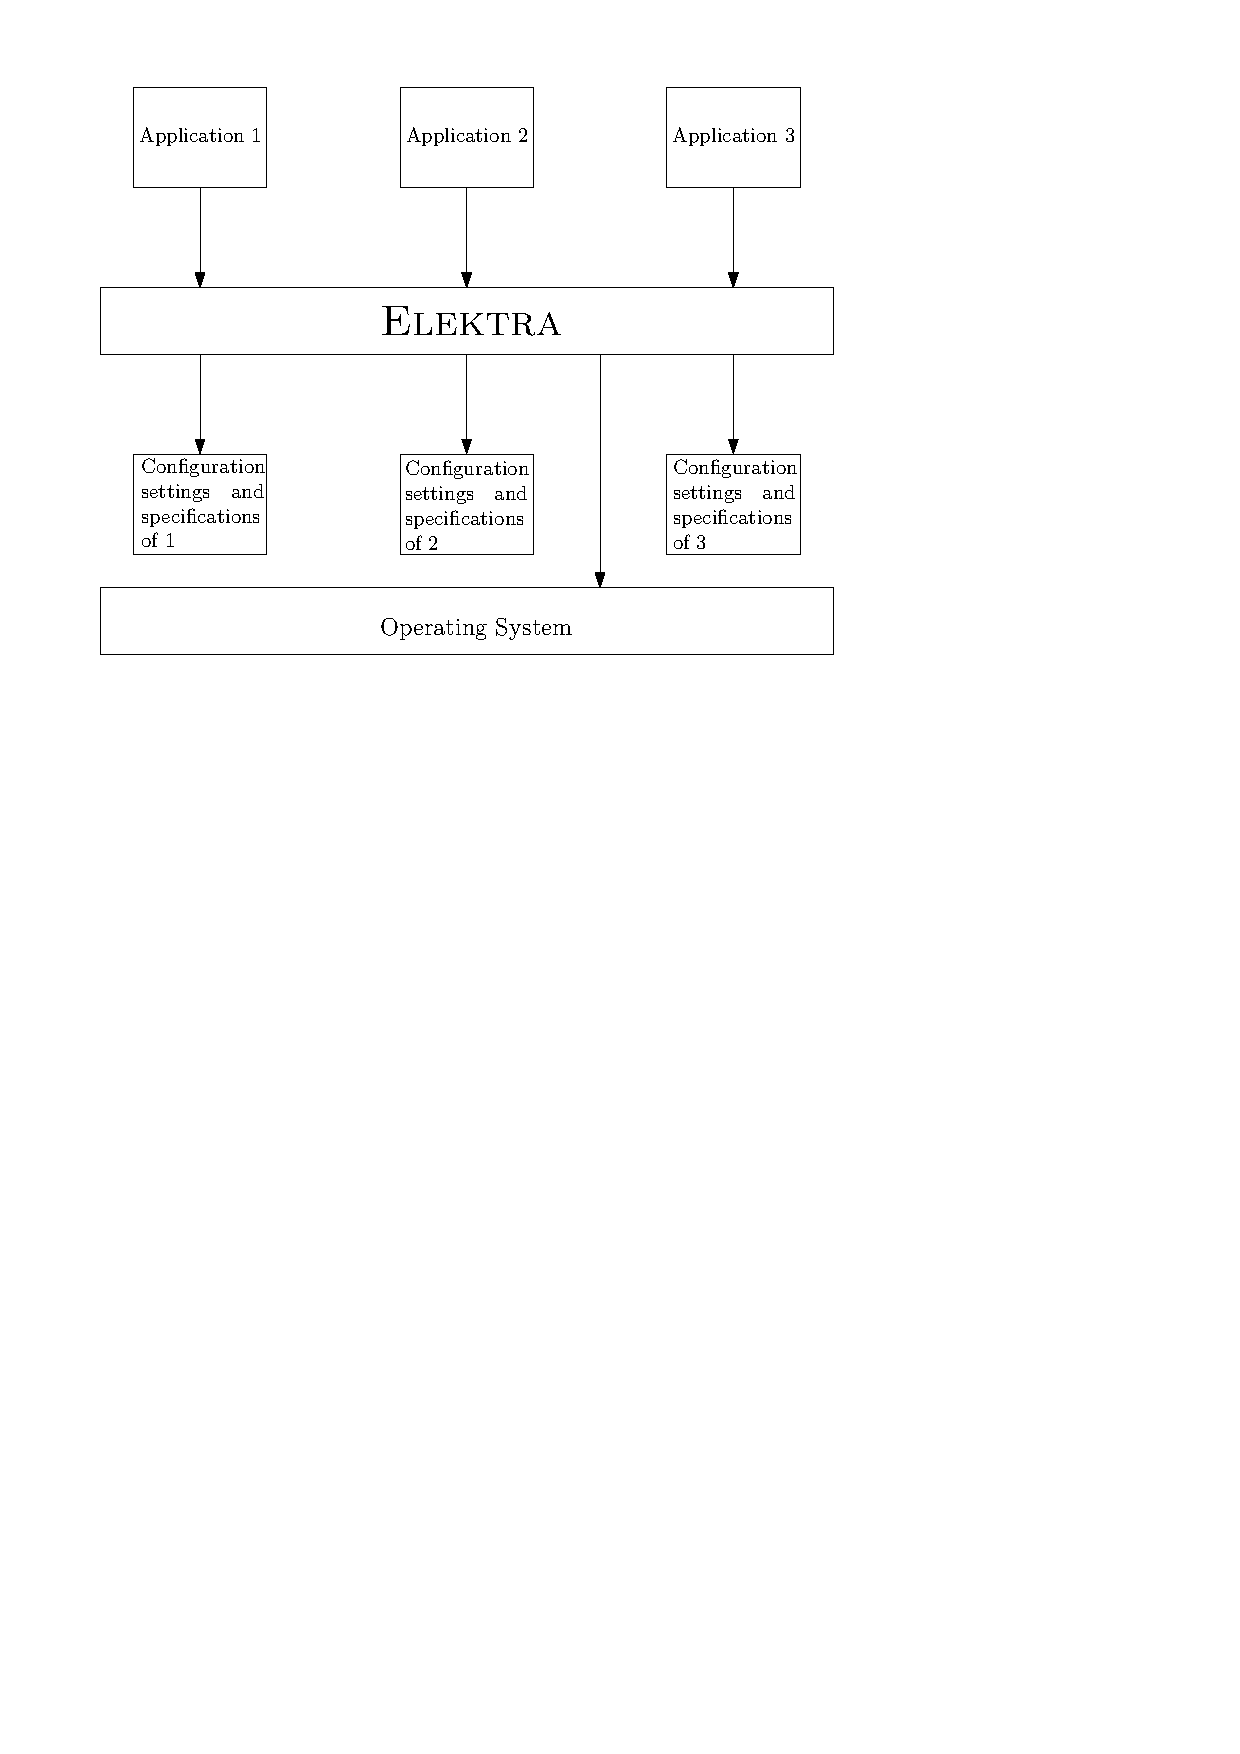
\includegraphics[width=\columnwidth]{wantsituation}
\caption[Wanted Situation.]{Wanted situation: \elektra{} as abstraction layer for configuration access of applications. We only need $3+4=7$ configuration accesses.}
\label{fig:wantsituation}
\end{figure}

Applications need to participate in the abstraction layer.
Therefore, we have to pursue \goalref{frontends} to give developers attractive solutions.

As stated in \goalref{abstraction}, we propose to unify configuration access via \elektra{Lib}.
To avoid losing any flexibility or modularity, we introduce the configuration specification language \elektra{Spec}, which enables applications to specify individual needs.%
{\parfillskip=0pt plus .8\textwidth \emergencystretch=.5\textwidth \par}

From our studies we found that fixed configuration specification languages are too limited to serve different domains~\cite{gunther2012software,berger2013survey,magableh2010primitive,friedrich1999consistency}.
Instead we propose a \empha{modular configuration specification language} that allows individual domains and applications to define their own extensions for the modular configuration specification language.
Only application-specific languages are suitable to specify configuration access for specific needs of individual applications.
As shown in Figure~\ref{fig:abstraction}, the modular configuration specification language is implemented by a chain of plugins.
Plugins support customized configuration validation and applications-specific functionality.


\begin{figure}[htp]
\centering
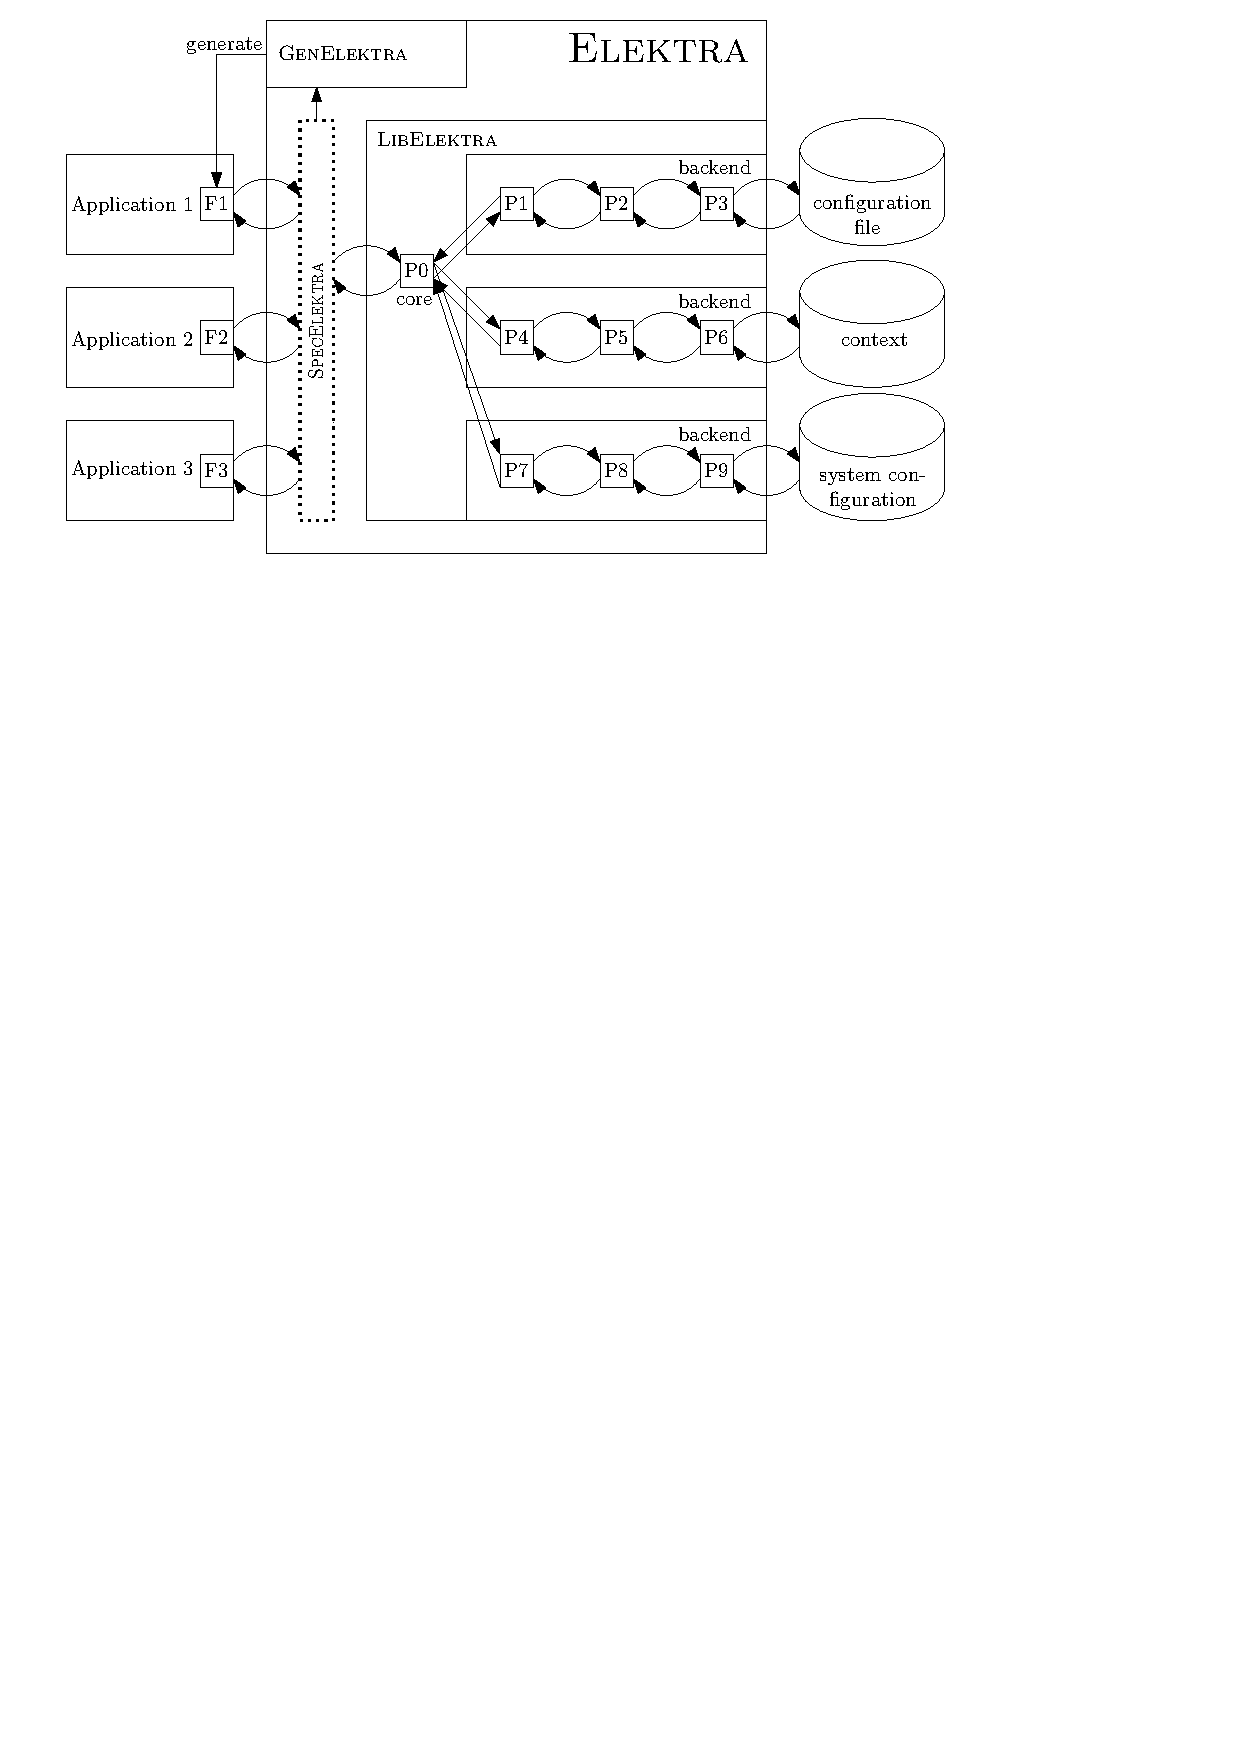
\includegraphics[width=\columnwidth]{abstraction}
\caption[\elektra{}'s Abstraction.]{\elektra{Lib} consists of backends that are built up by plugins.
Plugins contain application-specific or generic source code.
F? are frontends, which can be generated by \elektra{Gen} as shown for F1.
The other arrows indicate data flow of configuration settings and specifications.
P? are plugins nested in backends, and in this example, with P0 being part of every backend.}
\label{fig:abstraction}
\end{figure}

As main use case, extensions to the configuration specification language are used to build customized configuration access.
It is up to the designer of the extensions to put focus on context awareness or configuration validation.
In our book, our extensions focus towards context awareness, as described by \goalref{context}.
Because of \elektra{Spec}'s modularity and extensibility, \elektra{} supports specific requirements how to validate or derive configuration settings, without adding complexity to applications not needing such language constructs.

\begin{example}
Applications with a complex module system need a new language construct that is implemented using a constraint solver~\cite{fruhwirth2003essentials} to find optimal instantiations for the application's modules.
\end{example}

To demonstrate the usefulness of the modular configuration specification language \elektra{Spec}, we designed and built several language extensions with focus on context-aware configuration.
Together with \elektra{}, which enables every application to access configuration settings of the system and any other application, we leverage more context for configuration.
\elektra{Spec} can be seen as a glue language that is neutral to both programming languages and execution environments.

\elektra{Spec} shall fully enable developers to specify all relevant parts of configuration access.
Relevant parts include validity, transformation, context awareness, etc.
\begin{example}
\label{ex:introduction-solution}
To solve the problems of \exref{introduction-openldap-crash} on page~\pageref{ex:introduction-openldap-crash}, we specify:

\begin{code}[morekeywords={next}]
[slapd/threads/listener]
  check/range:=1,2,4,8,16
  context:=/slapd/threads/%cpu%/listener
  default:=1
  description:=One thread is adequate for up to 16 CPU cores.
  type:=long
\end{code}


Instead of calling the configuration setting ^listener-threads^, we give it a unique name, written in ^[]^.
The name makes the configuration setting and specification accessible in the whole system.
We use the hierarchy separator ^/^ that gives us flexibility when configuration settings are extended.
The other lines, which use ^:=^, are \empha[property]{properties} of this configuration specification.
All properties together fully specify access to this configuration setting.
Line~2 describes that only 5 values are valid, avoiding surprises and crashes.
Line~3 specifies that the configuration setting shall be contextually dependent on the number of CPUs available in the system.
The string ^%cpu%^ is a placeholder that is replaced with the current number of CPUs by a plugin.
We can create a mapping from the number of CPUs to the respective configuration values.
The resulting configuration value of this mapping then utilizes all CPUs.
If the calculation fails, for example, because the number of CPUs is unknown on that system or no mapping is available, we use the default value, which is ^1^ (line~4).
The last line specifies the data type for code generation with \elektra{Gen}.
\end{example}

Overall, \elektra{} aims at creating a better abstraction of local configuration access for applications.
The abstraction mitigates the configuration integration problem and enables users to program local configuration access for their needs.
This novel way of programming empowers developers, system administrators, and end users to:
\begin{enumerate}
 \item ensure validity of configuration settings in terms of the context,
 \item calculate default values honoring the context, and
 \item enable introspection of the resulting configuration settings and specifications.
\end{enumerate}
The enriched context awareness and improved configuration validation capabilities will be facilitated to exclude the possibility of some kinds of misconfiguration.

We claim that with such a simple specification language, accessing configuration settings and specifications for any participating application improves the goals \ref{goal:abstraction}, \ref{goal:context}, \ref{goal:frontends}, and the requirements unveiled in Goal~\ref{goal:requirements}.
As a result of the context awareness, we improve usability:
Applications will have more context-aware configurations.%
{\parfillskip=0pt plus .8\textwidth \emergencystretch=.2\textwidth \par}











\section{Structure, Research Questions, and Contributions}

After stating the main question and the overall contributions we will walk here chapter by chapter through the thesis to clarify research questions, contributions, and structure.

The main question of the book is:

\begin{restatable}{RQ}{rqMain}
Why is current FLOSS configuration access rarely context aware and how can we improve on the situation?%
\label{rq:main}
\end{restatable}


\citet{raab2014program,raab2015global,raab2015safe,raab2015kps,raab2016improving,raab2016unanticipated,raab2016persistent,raab2016elektra,raab2017introducing,raab2017challenges} contributed answers to the question.
\rqref{main} is both a design and research challenge:

\begin{enumerate}
\item research the challenges in context-aware configuration access,
\item solve the design problem, i.\,e., find the best candidate to tackle the challenges, and
\item research the implications of the design we have chosen and evaluate if it improves on the configuration integration problem.
\end{enumerate}

The main contribution of this book are improvements on context awareness for configuration access, resulting in more context-aware configurations:
\begin{itemize}
\item We enable software to be more context aware via their configuration settings~\cite{raab2015kps}.
\item We enable developers and system administrators to improve context awareness without a change of their programming language and, with some limitations, without any change of the applications' source code~\cite{raab2016unanticipated}.
\item We improve introspection and debugging of configuration access. Our contributions are steps towards a no-futz system~\cite{holland2001nofutz}.
\item We analyze the performance situation of configuration accesses and suggest simple but effective optimization techniques~\cite{raab2014program}.
\item We improve abstraction and modularization using a modular configuration specification language that supports context-aware configuration~\cite{raab2016improving}.
\item As contribution to the FLOSS ecosystem, \elektra{} is available as free software at:
\url{https://www.libelektra.org}.
\end{itemize}



\subsection{Terminology and Background}

We establish terminology and background in \chapref{background}.
We surveyed literature in misconfiguration, configuration specification languages, context-oriented programming, and context-aware configurations, answering the following research questions:

\begin{restatable}{RQ}{rqBackground}
 \label{rq:background}
What is configuration, context, and context-aware configuration?
\end{restatable}

\begin{restatable}{RQsub}{rqBackgroundViewpoints}
 \label{rq:background-viewpoints}
What are the viewpoints of context-aware configuration?
\end{restatable}

\begin{contribution}
We consistently establish terminology, viewpoints, and background for context-aware configuration.
At least three viewpoints, i.\,e.\ sensors, users, and time, constitute the distinction between ordinary and context-aware configurations.
\end{contribution}

\begin{restatable}{RQsub}{rqBackgroundSpecificationLanguages}
 \label{rq:background-specification-languages}
 Which configuration specification languages are suitable to improve configuration access of FLOSS applications?
\end{restatable}

\begin{contribution}
Despite conducting a systematic, large-scale literature survey, we did not find any configuration specification language that focused on the configuration integration problem.
\end{contribution}

\subsection{Relevance to the Community}

While there is generally no doubt about the presence of many problems surrounding misconfiguration, the analysis of their details proves to be difficult and is still ongoing.
We pioneered new aspects, framed as the configuration integration problem, mainly ourselves.
In \chapref{motivation}, we describe how we unveiled these challenges.
We report on a large-scale source code analysis, a questionnaire survey, and \elektra{}'s community experience, answering the question:

\begin{restatable}{RQ}{rqMotivation}
Why do FLOSS applications lack \empha{context awareness} and \empha{configuration validation} for configuration settings and what are the challenges in providing them?
 \label{rq:motivation}
\end{restatable}

For the empirical source code analysis we classified 2,683 call sites of configuration accesses in 16 real-world applications encompassing 50 million lines of code.
Additionally a questionnaire was shown to 672 persons, 286 of these persons started to answer, 162 of these persons completed the questionnaire, and 116 persons handed their email addresses to be contacted by us afterwards~\cite{raab2017challenges}.

\begin{contribution}
We found many different problems causing the described symptoms and collected requirements for potential solutions.
\end{contribution}

\begin{restatable}{RQsub}{rqMotivationObservation}
Which problems in configuration access are observed while developing FLOSS with state-of-the-art techniques?%
\label{rq:motivation-observation}
\end{restatable}

\begin{contribution}
We observed different maintenance problems such as duplication and inconsistencies of configuration accesses and settings.
\end{contribution}

\begin{restatable}{RQsub}{rqMotivationCurrentState}
What is the current state of configuration access in FLOSS?%
\label{rq:motivation-current-state}
\end{restatable}

\begin{contribution}
We found that different types of execution environments are equally popular and unveiled details about why the decision, which one to use, is often arbitrary.
\end{contribution}

\begin{restatable}{RQsub}{rqMotivationContext}
Which proportion of configuration accesses is already context aware or can be made so without any source code changes?%
\label{rq:motivation-context}
\end{restatable}

\begin{contribution}
We learned that developers are striving to support context awareness.
In other cases, configuration accesses were used as if they were context aware, even though they are not.
We found that such configuration accesses provide potential for run-time adaptations without modifying the source code of the applications.
\end{contribution}

In the following sub-questions from \rqref{motivation-context}, we mainly looked at the configuration access API ^getenv^.
We expected ^getenv^ to be widely adopted because of its standardization.
We present the adoption rate of ^getenv^ and show that non-context-aware configuration accesses exist in the source code of applications:

\begin{restatable}{RQsubsub}{rqMotivationContextUsage}
What are the usage patterns of \texttt{getenv} invocations in the source code of popular applications?%
\label{rq:motivation-context-usage}
\end{restatable}

\begin{contribution}
In a source code analysis of 16 FLOSS applications we found that a particular kind of configuration accesses, namely the ^getenv^ API, is used pervasively in 2,683 call sites~\cite{raab2017introducing}.
It is inevitable that in many of these places the context is forgotten: we found confirmed cases.
\end{contribution}

We have to show that these configuration accesses are used in a way exploitable for run-time adaptations:

\begin{restatable}{RQsubsub}{rqMotivationContextRepeat}
How often is \texttt{getenv} repeatedly used at run-time?%
\label{rq:motivation-context-repeat}
\end{restatable}

\begin{contribution}
We found ^getenv^ invocations to happen extensively across all studied applications.
Many ^getenv^ invocations happen repeatedly and can be exploited for improving context awareness.
\end{contribution}

Putting the pieces of \chapref{motivation} together, we compiled a list of requirements to improve on the configuration integration problem:

\begin{restatable}{RQsub}{rqMotivationChallenges}
What are the challenges and requirements in providing configuration access for context-aware configuration?%
\label{rq:motivation-challenges}
\end{restatable}

\begin{contribution}
Overall, \chapref{motivation} contributes towards a better understanding of the problem and unveils the first list of empirically founded requirements for context-aware configuration access.
\end{contribution}


\subsection{\textsc{Elektra}}

\addtocounter{RQ}{1}

In~\chapref{approach}, we formalize a model of \elektra{}'s central parts.
\elektra{} introduces a novel form of abstraction yielding context-aware configuration.

\begin{contribution}
\chapref{approach} contains the first formalization of a framework to access context-aware configuration.
It includes a simple proof for eliding an instantiation of misconfiguration, namely missing configuration settings.
\end{contribution}

Different from~\chapref{approach}, the next two chapters \ref{chapter:frontend} and \ref{chapter:backend} will elaborate on why this model fulfills the requirements and how the abstractions work in practice.


\subsection{Frontends}

\intro[frontend]{Frontends} are the parts of configuration accesses that are compiled into applications.
Every application accessing configuration settings needs some kind of frontend.
At minimum the frontend consists of configuration access API invocations, at maximum applications include everything found in configuration libraries.
In \elektra{}, frontends are minimal or generated with \elektra{Gen}.

Most developers include source code within their applications that implements configuration access.
Configuration transformations and validations within these frontends are an important factor of the configuration integration problem.
In \chapref{frontend}, we discuss how we simplify frontend code with context-aware APIs, answering the following research questions:%
{\parfillskip=0pt plus .8\textwidth \emergencystretch=.2\textwidth \par}

\begin{restatable}{RQ}{rqFrontend}
 \label{rq:frontend-requirement}
 Which concepts are needed for context-aware frontends to fulfill the requirements as unveiled in \chapref{motivation}?
\end{restatable}

\begin{restatable}{RQsub}{rqFrontendDesignDecisions}
 \label{rq:frontend-design-decisions}
 What is the design space for context-aware frontends?
\end{restatable}

\begin{restatable}{RQsub}{rqFrontendTradeOff}
 \label{rq:frontend-trade-off}
Which implementation technique for implementing context-aware frontends has the best trade-off for time versus space?
\end{restatable}

\begin{restatable}{RQsub}{rqFrontendConcurrent}
 \label{rq:frontend-concurrent}
 How can we improve on the usability of context-aware frontends if being used concurrently from several threads?
\end{restatable}

\begin{restatable}{RQsub}{rqFrontendUsability}
 \label{rq:frontend-usability}
 How can we share context between applications?
\end{restatable}

\begin{contribution}
We establish a context-aware frontend that:
\begin{enumerate}
 \item fulfills the requirements unveiled in \chapref{motivation} and integrates context-oriented programming with the execution environment,
 \item has zero overhead for read access even if used in multi-threaded applications, and
 \item guarantees some properties of configuration specifications, improving on the configuration integration problem.
\end{enumerate}
\end{contribution}


\subsection{Backends}

\intro[backend]{Backends} are all parts of configuration access that are not part of the frontends.
Our implementation of the backends is \elektra{Lib}.
Different to the frontends, the backends are shared among all applications in a system.

In \chapref{backend}, we will investigate parts of the configuration integration problem that cannot be solved by frontends.
In particular, problems that involve several applications written in different programming languages need a solution within the backends.

\begin{restatable}{RQ}{rqBackend}
Which concepts are needed for context-aware backends to fulfill the requirements as unveiled in \chapref{motivation}?%
\label{rq:backend}
\end{restatable}

\begin{restatable}{RQsub}{rqBackendDesignDecisions}
What is the design space for abstractions of context-aware configuration in backends?%
\label{rq:backend-design-decisions}
\end{restatable}

\begin{restatable}{RQsub}{rqBackendContextLookup}
How can we enable context awareness in backends without support from frontends?%
\label{rq:backend-context-lookup}
\end{restatable}

\begin{restatable}{RQsub}{rqBackendModularAbstractions}
\label{rq:backend-modular-abstractions}
Which abstractions retain and improve modularity of configuration access in FLOSS applications?
\end{restatable}


\begin{restatable}{RQsub}{rqBackendContextUnmodified}
 \label{rq:backend-context-unmodified}
 Which techniques enable applications to become more context aware without any changes in the source code?
\end{restatable}

\begin{contribution}
The main results in \chapref{backend} are:
\begin{enumerate}
\item Using simple specifications, \elektra{} provides programmable backends fulfilling the requirements unveiled in \chapref{motivation}.
\item Abstractions enable us to keep the current modularity of FLOSS applications, and even extend it for configuration access.
\item \elektra{} allows legacy applications to become context aware without any source code modifications.
\item It is possible to share configuration settings, specifications, and contexts across the whole system.
\end{enumerate}
\end{contribution}

\subsection{Implications and Open Topics}

Even though each individual part of our implementation is lightweight because of \elektra{}'s modularity, altogether we propose a rather heavyweight, system-oriented abstraction.
One must carefully consider whether the advantages outweigh the risks.

In \chapref{implications}, we will consider the implications \elektra{} has on the FLOSS ecosystem.
The implications are complex and sometimes, not surprisingly, beyond the problems we initially wanted to tackle.
We will reflect on experiences with users and case studies:

\begin{restatable}{RQ}{rqImplication}
What are the risks and implications of introducing \elektra{}?%
\label{rq:implication}
\end{restatable}

\begin{restatable}{RQsub}{rqImplicationAdministration}
Which risks and implications does \elektra{} have for administrating configuration settings?%
\label{rq:implication-administration}
\end{restatable}

\begin{contribution}
A unified interface for configuration settings brings control to the system administrator.
On the downside, system administrators need to learn \elektra{}'s concepts.
We demonstrate that our solution is applicable to a variety of use cases.
We show that \elektra{} is not only feasible, but also practical and seamlessly supports debugging and introspection of configuration settings and specifications.
\end{contribution}

\begin{restatable}{RQsub}{rqImplicationDevelopmentTime}
How does \elektra{} influence risks of development and time effort if used in a large real-world project?%
\label{rq:implication-development-time}
\end{restatable}

\begin{restatable}{RQsub}{rqImplicationEmbedded}
\label{rq:implication-embedded}
Which features are elegantly realizable in \elektra{} to configure non-trivial embedded systems?
\end{restatable}

\begin{contribution}
We were able to use \elektra{} within several large real-world and embedded projects successfully.
Due to \elektra{}'s extensibility and due to reuse of already existing components, developers saved time.
On the downside, some additional complexity needs to be mastered.
\elektra{Spec} enables us to defer decisions, reducing some risks.
\end{contribution}

\begin{restatable}{RQsub}{rqImplicationDebuggingSupport}
\label{rq:implication-debugging-support}
How can we improve debugging support of context-oriented programs?
\end{restatable}

\begin{contribution}
We present debugging techniques that deal with additional flexibility introduced by context awareness.
\end{contribution}

\begin{restatable}{RQsub}{rqImplicationSecurity}
What are the risks and implications on security, safety, and quality in systems using \elektra{}?%
\label{rq:implication-security}
\end{restatable}

\begin{restatable}{RQsubsub}{rqImplicationMetrics}
What are the source code metrics of \elektra{} and who develops \elektra{}?%
\label{rq:implication-metrics}
\end{restatable}

\begin{restatable}{RQsubsub}{rqImplicationMisconfiguration}
What are the implications of \elektra{} on misconfiguration?%
\label{rq:implication-misconfiguration}
\end{restatable}

\begin{contribution}
In \chapref{implications}, we demonstrate the practicality and generality of our solution by porting different applications to \elektra{}.
We cannot claim the resulting systems to be always more secure and free of misconfiguration.
Nevertheless, we argue that some classes of misconfiguration get much more unlikely with \elektra{}.
Some classes of misconfigurations would only be possible because of bugs in the implementation and not due to operator mistakes.
Furthermore, we argue that a centralized implementation improves on quality, reliability, and security.
We are positive that \elektra{} raises the bar for future configuration libraries.
\end{contribution}


\subsection{Evaluation}

In \chapref{evaluation}, we conduct benchmarks and measure further software characteristics in applications using \elektra{}, answering the research question:

\begin{restatable}{RQ}{rqEvaluation}
Which software characteristics change if \elektra{} is applied?%
\label{rq:evaluation}
\end{restatable}

\begin{restatable}{RQsub}{rqEvaluationFrontend}
\label{rq:evaluation-frontend}
What are the performance characteristics for applications specifically programmed for \elektra{}?
\end{restatable}

\begin{restatable}{RQsubsub}{rqEvaluationFrontendPerformance}
\label{rq:evaluation-frontend-performance}
How much can we improve the performance of configuration access using context-oriented programming?
\end{restatable}

Different from non-context-aware applications, context-aware applications need to track all \empha[context change]{context changes} occurring in the system.
Thus we focused our investigations to measuring overhead of context changes.

\begin{restatable}{RQsubsub}{rqEvaluationFrontendMultiThreadOverhead}
\label{rq:evaluation-frontend-multi-thread-overhead}
What is the overhead of context changes in an embedded, multi-threaded use case?
\end{restatable}

\begin{restatable}{RQsubsub}{rqEvaluationFrontendPerformanceComparison}
\label{rq:evaluation-frontend-performance-comparison}
What is the cost of \elektra{}'s individual operations?
\end{restatable}

\begin{restatable}{RQsubsub}{rqEvaluationFrontendRessourceUtilization}
\label{rq:evaluation-frontend-resource-utilization}
How is \elektra{}'s resource utilization of hard disk storage?
\end{restatable}

\begin{restatable}{RQsubsub}{rqEvaluationFrontendComparison}
\label{rq:evaluation-frontend-comparison}
What are the performance trade-offs towards high-level abstractions for context changes?
\end{restatable}

\begin{restatable}{RQsubsub}{rqEvaluationFrontendEmbeddedActivation}
What is the overhead of high-level abstractions for context changes in embedded scenarios?%
\label{rq:evaluation-frontend-embedded-activation}
\end{restatable}

The contribution of \rqref{evaluation-frontend} is:

\begin{contribution}
All overheads are either constant or increase linearly in execution time.
Although some high-level abstractions have considerably more overhead, even context changes every few milliseconds have little impact.
\end{contribution}

\begin{restatable}{RQsub}{rqComparisonFrontendBackend}
What are the considerations to implement a feature in the frontends versus in the backends?%
\label{rq:comparison-frontend-backend}
\end{restatable}

\begin{contribution}
While there is a difference in overhead, we nevertheless recommend implementing virtually all features---except thread-safe, dynamically-scoped, context-aware configuration access APIs---in backends.
Only then the features can be interpreted dynamically and can be easily shared between applications in different programming languages.
\end{contribution}

\begin{restatable}{RQsub}{rqOverheadModularity}
\label{rq:overhead-modularity}
What is the overhead of \elektra{}'s modular abstractions?
\end{restatable}

\begin{contribution}
The overhead does not give a reason to avoid modularity.
\end{contribution}

One of the main contributions is that completely unmodified applications (concerning the source code) can use \elektra{}.
Our assumption is that applications already have configurable behavioral variations.
The basic idea is to have a run-time system that computes which behavior variations shall be active to match the context.
We strive to answer the research questions:

\begin{restatable}{RQsub}{rqUnmodified}
What are the characteristics of a system in which context-unaware software was made more context aware without any modifications in the source code?%
\label{rq:unmodified}
\end{restatable}

\begin{restatable}{RQsubsub}{rqUnmodifiedWhich}
 \label{rq:unmodified-which}
How many \texttt{getenv} invocations can be exploited to improve context awareness without any modifications in the source code?
\end{restatable}

\begin{restatable}{RQsubsub}{rqUnmodifiedPractical}
\label{rq:unmodified-practical}
How can we practically make applications more context aware without any modifications in the source code?
\end{restatable}

\begin{restatable}{RQsubsub}{rqUnmodifiedOverhead}
\label{rq:unmodified-overhead}
What overhead occurs in applications intercepted by \elektra{}?
\end{restatable}

\begin{restatable}{RQsubsub}{rqUnmodifiedPerformance}
 \label{rq:unmodified-performance}
What is the performance implication that occurs on context changes?
\end{restatable}

The main contributions of \rqref{unmodified} and its sub-questions are:
\begin{contribution}
We collected profound evidence that \elektra{} improves context awareness in FLOSS applications even though we did not change a single line of source code in the respective applications~\cite{raab2017introducing}:
\begin{enumerate}
\item
No evaluation of context-aware applications was conducted before using such complex, large, and popular applications~\cite{raab2017introducing}.
The contributions are steps in the effort of understanding the software-engineering perspective of context-aware configuration.%
{\parfillskip=0pt \emergencystretch=.2\textwidth \par}

\item 
In a practical case study, with focus on Web browsers, we improved context awareness for flexible workplaces.
We conduct a software-engineering process in which we systematically improve context awareness without any source code modifications.

\end{enumerate}
\end{contribution}

\subsection{Related Work}

In \chapref{related} we will discuss related work.
As we will see, state-of-the-art techniques assume that applications need to be rewritten in architectures unusual for FLOSS.
We avoid this assumption and investigate in methods that can be realized for legacy applications.

\begin{restatable}{RQ}{rqRelated}
Why does related work not solve the configuration integration problem?
\end{restatable}

\subsection{Conclusion and Future Work}

Our work showed that it is feasible and practical that a high-level configuration specification language unifies configuration access and mitigates the configuration integration problem.
In \chapref{conclusion}, we will conclude the book with a discussion about the achieved goals.
In this light, we will elaborate on perspectives left open as future work.%
{\parfillskip=0pt \emergencystretch=.5\textwidth \par}

\pagebreak

Finally, we give a summary of the value our line of research has for the \empha[stakeholder]{stakeholders}:
\begin{description}
\item[Developers] get better frontends that enable them to directly work with variables that contain context-aware configuration.
With this higher level of abstraction, they do not have to care about configuration validation and context awareness within the application's source code.
Another main contribution to developers is \elektra{Spec} that allows them to define valid, context-aware configurations more concisely without bringing further dependences in the application's source code.%
{\parfillskip=0pt \emergencystretch=.5\textwidth \par}


\item[System administrators] get better tooling that allows them to introspect and change configuration settings without any syntactic hurdles and futzing.
\elektra{Spec} empowers them to understand and improve the validations and context awareness on a system level.
Our main contribution to system administrators is better user interfaces that make some kinds of misconfiguration much more unlikely.
Misconfiguration gets rejected earlier with better error messages.

\item[End users] mainly benefit from having more context awareness in applications.
Our main contribution to end users is that \elektra{} enables them to personalize every configuration setting for every context.
\end{description}
